% Options for packages loaded elsewhere
\PassOptionsToPackage{unicode}{hyperref}
\PassOptionsToPackage{hyphens}{url}
\PassOptionsToPackage{dvipsnames,svgnames,x11names}{xcolor}
%
\documentclass[
  ignorenonframetext,
]{beamer}
\usepackage{pgfpages}
\setbeamertemplate{caption}[numbered]
\setbeamertemplate{caption label separator}{: }
\setbeamercolor{caption name}{fg=normal text.fg}
\beamertemplatenavigationsymbolsempty
% Prevent slide breaks in the middle of a paragraph
\widowpenalties 1 10000
\raggedbottom
\setbeamertemplate{part page}{
  \centering
  \begin{beamercolorbox}[sep=16pt,center]{part title}
    \usebeamerfont{part title}\insertpart\par
  \end{beamercolorbox}
}
\setbeamertemplate{section page}{
  \centering
  \begin{beamercolorbox}[sep=12pt,center]{part title}
    \usebeamerfont{section title}\insertsection\par
  \end{beamercolorbox}
}
\setbeamertemplate{subsection page}{
  \centering
  \begin{beamercolorbox}[sep=8pt,center]{part title}
    \usebeamerfont{subsection title}\insertsubsection\par
  \end{beamercolorbox}
}
\AtBeginPart{
  \frame{\partpage}
}
\AtBeginSection{
  \ifbibliography
  \else
    \frame{\sectionpage}
  \fi
}
\AtBeginSubsection{
  \frame{\subsectionpage}
}
\usepackage{amsmath,amssymb}
\usepackage{lmodern}
\usepackage{iftex}
\ifPDFTeX
  \usepackage[T1]{fontenc}
  \usepackage[utf8]{inputenc}
  \usepackage{textcomp} % provide euro and other symbols
\else % if luatex or xetex
  \usepackage{unicode-math}
  \defaultfontfeatures{Scale=MatchLowercase}
  \defaultfontfeatures[\rmfamily]{Ligatures=TeX,Scale=1}
\fi
% Use upquote if available, for straight quotes in verbatim environments
\IfFileExists{upquote.sty}{\usepackage{upquote}}{}
\IfFileExists{microtype.sty}{% use microtype if available
  \usepackage[]{microtype}
  \UseMicrotypeSet[protrusion]{basicmath} % disable protrusion for tt fonts
}{}
\makeatletter
\@ifundefined{KOMAClassName}{% if non-KOMA class
  \IfFileExists{parskip.sty}{%
    \usepackage{parskip}
  }{% else
    \setlength{\parindent}{0pt}
    \setlength{\parskip}{6pt plus 2pt minus 1pt}}
}{% if KOMA class
  \KOMAoptions{parskip=half}}
\makeatother
\usepackage{xcolor}
\newif\ifbibliography
\usepackage{color}
\usepackage{fancyvrb}
\newcommand{\VerbBar}{|}
\newcommand{\VERB}{\Verb[commandchars=\\\{\}]}
\DefineVerbatimEnvironment{Highlighting}{Verbatim}{commandchars=\\\{\}}
% Add ',fontsize=\small' for more characters per line
\usepackage{framed}
\definecolor{shadecolor}{RGB}{248,248,248}
\newenvironment{Shaded}{\begin{snugshade}}{\end{snugshade}}
\newcommand{\AlertTok}[1]{\textcolor[rgb]{0.94,0.16,0.16}{#1}}
\newcommand{\AnnotationTok}[1]{\textcolor[rgb]{0.56,0.35,0.01}{\textbf{\textit{#1}}}}
\newcommand{\AttributeTok}[1]{\textcolor[rgb]{0.77,0.63,0.00}{#1}}
\newcommand{\BaseNTok}[1]{\textcolor[rgb]{0.00,0.00,0.81}{#1}}
\newcommand{\BuiltInTok}[1]{#1}
\newcommand{\CharTok}[1]{\textcolor[rgb]{0.31,0.60,0.02}{#1}}
\newcommand{\CommentTok}[1]{\textcolor[rgb]{0.56,0.35,0.01}{\textit{#1}}}
\newcommand{\CommentVarTok}[1]{\textcolor[rgb]{0.56,0.35,0.01}{\textbf{\textit{#1}}}}
\newcommand{\ConstantTok}[1]{\textcolor[rgb]{0.00,0.00,0.00}{#1}}
\newcommand{\ControlFlowTok}[1]{\textcolor[rgb]{0.13,0.29,0.53}{\textbf{#1}}}
\newcommand{\DataTypeTok}[1]{\textcolor[rgb]{0.13,0.29,0.53}{#1}}
\newcommand{\DecValTok}[1]{\textcolor[rgb]{0.00,0.00,0.81}{#1}}
\newcommand{\DocumentationTok}[1]{\textcolor[rgb]{0.56,0.35,0.01}{\textbf{\textit{#1}}}}
\newcommand{\ErrorTok}[1]{\textcolor[rgb]{0.64,0.00,0.00}{\textbf{#1}}}
\newcommand{\ExtensionTok}[1]{#1}
\newcommand{\FloatTok}[1]{\textcolor[rgb]{0.00,0.00,0.81}{#1}}
\newcommand{\FunctionTok}[1]{\textcolor[rgb]{0.00,0.00,0.00}{#1}}
\newcommand{\ImportTok}[1]{#1}
\newcommand{\InformationTok}[1]{\textcolor[rgb]{0.56,0.35,0.01}{\textbf{\textit{#1}}}}
\newcommand{\KeywordTok}[1]{\textcolor[rgb]{0.13,0.29,0.53}{\textbf{#1}}}
\newcommand{\NormalTok}[1]{#1}
\newcommand{\OperatorTok}[1]{\textcolor[rgb]{0.81,0.36,0.00}{\textbf{#1}}}
\newcommand{\OtherTok}[1]{\textcolor[rgb]{0.56,0.35,0.01}{#1}}
\newcommand{\PreprocessorTok}[1]{\textcolor[rgb]{0.56,0.35,0.01}{\textit{#1}}}
\newcommand{\RegionMarkerTok}[1]{#1}
\newcommand{\SpecialCharTok}[1]{\textcolor[rgb]{0.00,0.00,0.00}{#1}}
\newcommand{\SpecialStringTok}[1]{\textcolor[rgb]{0.31,0.60,0.02}{#1}}
\newcommand{\StringTok}[1]{\textcolor[rgb]{0.31,0.60,0.02}{#1}}
\newcommand{\VariableTok}[1]{\textcolor[rgb]{0.00,0.00,0.00}{#1}}
\newcommand{\VerbatimStringTok}[1]{\textcolor[rgb]{0.31,0.60,0.02}{#1}}
\newcommand{\WarningTok}[1]{\textcolor[rgb]{0.56,0.35,0.01}{\textbf{\textit{#1}}}}
\usepackage{graphicx}
\makeatletter
\def\maxwidth{\ifdim\Gin@nat@width>\linewidth\linewidth\else\Gin@nat@width\fi}
\def\maxheight{\ifdim\Gin@nat@height>\textheight\textheight\else\Gin@nat@height\fi}
\makeatother
% Scale images if necessary, so that they will not overflow the page
% margins by default, and it is still possible to overwrite the defaults
% using explicit options in \includegraphics[width, height, ...]{}
\setkeys{Gin}{width=\maxwidth,height=\maxheight,keepaspectratio}
% Set default figure placement to htbp
\makeatletter
\def\fps@figure{htbp}
\makeatother
\setlength{\emergencystretch}{3em} % prevent overfull lines
\providecommand{\tightlist}{%
  \setlength{\itemsep}{0pt}\setlength{\parskip}{0pt}}
\setcounter{secnumdepth}{-\maxdimen} % remove section numbering
\usepackage{graphicx}
\usepackage{bm}
\usepackage{array}
\usepackage{amsmath}
\usepackage{amsthm}
\usepackage{amsfonts}
\usepackage{amssymb}
\usepackage{tikz-cd}
\usepackage{url}
\definecolor{foreground}{RGB}{255,255,255}
\definecolor{background}{RGB}{34,28,54}
\definecolor{title}{RGB}{105,165,255}
\definecolor{gray}{RGB}{175,175,175}
\definecolor{lightgray}{RGB}{225,225,225}
\definecolor{subtitle}{RGB}{232,234,255}
\definecolor{hilight}{RGB}{112,224,255}
\definecolor{vhilight}{RGB}{255,111,207}
\setbeamertemplate{footline}[page number]
\ifLuaTeX
  \usepackage{selnolig}  % disable illegal ligatures
\fi
\IfFileExists{bookmark.sty}{\usepackage{bookmark}}{\usepackage{hyperref}}
\IfFileExists{xurl.sty}{\usepackage{xurl}}{} % add URL line breaks if available
\urlstyle{same} % disable monospaced font for URLs
\hypersetup{
  pdftitle={STAT 528 - Advanced Regression Analysis II},
  pdfauthor={Binary response regression (part I)},
  colorlinks=true,
  linkcolor={Maroon},
  filecolor={Maroon},
  citecolor={Blue},
  urlcolor={blue},
  pdfcreator={LaTeX via pandoc}}

\title{STAT 528 - Advanced Regression Analysis II}
\author{Binary response regression (part I)}
\date{}
\institute{Daniel J. Eck\\
Department of Statistics\\
University of Illinois}

\begin{document}
\frame{\titlepage}

\begin{frame}
\newcommand{\R}{\mathbb{R}}
\newcommand{\Prob}{\mathbb{P}}
\newcommand{\Proj}{\textbf{P}}
\newcommand{\Hcal}{\mathcal{H}}
\newcommand{\rootn}{\sqrt{n}}
\newcommand{\p}{\mathbf{p}}
\newcommand{\E}{\text{E}}
\newcommand{\Var}{\text{Var}}
\newcommand{\Cov}{\text{Cov}}
\newcommand{\pibf}{\bm{\pi}}
\newcommand{\logit}{\text{logit}}

\newtheorem{cor}{Corollary}
\newtheorem{lem}{Lemma}
\newtheorem{thm}{Theorem}
\newtheorem{defn}{Definition}
\newtheorem{prop}{Proposition}
\end{frame}

\begin{frame}{Last time}
\protect\hypertarget{last-time}{}
\begin{itemize}
\tightlist
\item
  Optimization
\item
  Sufficiency
\item
  Maximum Entropy
\item
  Wrap-up
\end{itemize}
\end{frame}

\begin{frame}{Learning Objectives Today}
\protect\hypertarget{learning-objectives-today}{}
\begin{itemize}
\tightlist
\item
  logistic regression
\item
  data analysis
\item
  connecting theory to application
\end{itemize}
\end{frame}

\begin{frame}{Background}
\protect\hypertarget{background}{}
We suppose that we have a sample of data \((y_i,x_i)\),
\(i = 1,\ldots, n\) where

\begin{itemize}
\tightlist
\item
  \(y_i\) is a scalar response variable
\item
  \(x_i\) is a vector of predictors.
\end{itemize}

Recall from the exponential family notes that the log likelihood of the
exponential family is of the form \begin{equation} \label{expolog}
    l(\theta) = \langle y, \theta \rangle - c(\theta),
\end{equation} where

\begin{itemize}
\tightlist
\item
  \(y \in \mathbb{R}^n\) is a vector statistic having components
\item
  \(\theta \in \mathbb{R}^n\) is the canonical parameter vector.
\end{itemize}

In those notes \(\theta\) is unconstrained and the likelihood
\eqref{expolog} corresponds to a saturated regression model, one
parameter for every observation.
\end{frame}

\begin{frame}{}
\protect\hypertarget{section}{}
A canonical linear submodel of an exponential family is a submodel
having parameterization \[
  \theta = M\beta,
\] and log likelihood \begin{equation} \label{subloglike}
  l(\beta) = \langle M'y, \beta \rangle - c(M\beta).
\end{equation}

In an exponential family GLM, the saturated model canonical parameter
vector \(\theta\) is ``linked'\,' to the saturated model mean value
parameter vector through the change-of-parameter mappings \(g(\theta)\).

\vspace{12pt}

We can write \[
 \mu = \text{E}_\theta(Y) = g(M\beta) 
\] which implies that we can write \[
  g^{-1}\left(\text{E}_\theta(Y)\right) = M\beta.
\]

\vspace{12pt}

This is the basis of exponential family generalized linear models with
link function \(g^{-1}\).
\end{frame}

\begin{frame}{Logistic regression model}
\protect\hypertarget{logistic-regression-model}{}
\vspace{12pt}

The logistic regression model is one of the most widely used and studied
GLMs in practice.

\vspace{12pt}

It is {[}one of{]} the most important model for binary response data,
being commonly used for a wide variety of applications.

\vspace{12pt}

The logistic regression model is used for analyzing a binary response
variable, \(y_i \in \{0,1\}\) where a \(1\) encodes a ``success'' and a
0 encodes a ``failure.''

\vspace{12pt}

The logistic regression model allows for users to model the probability
of success as a function of covariates.
\end{frame}

\begin{frame}{}
\protect\hypertarget{section-1}{}
For a binary response variable \(Y\) and a vector of predictors \(X\),
let \[
  \pi(x) = P(Y = 1|X = x). 
\]\\
The logistic regression model is then \begin{equation} \label{logit}
  \pi(x) = P(Y = 1|X = x) = \frac{\exp(x'\beta)}{1 + \exp(x'\beta)}.
\end{equation} Equivalently, the \emph{logit} (log-odds) of the response
variable has a linear relationship in the canonical submodel parameters:
\[
  \text{logit}(\pi(x)) = \log\left(\frac{\pi(x)}{1 - \pi(x)}\right) =  x^T\beta.
\] In vector notation, we can express the above as \[
  \bm{\pi}= \frac{\exp(M\beta)}{1 + \exp(M\beta)} = \frac{1}{1 + \exp(-M\beta)} \quad \text{and} \quad 
    \text{logit}(\bm{\pi}) = M\beta
\] where the above \(\exp(\cdot)\) and logit\((\cdot)\) operations are
understood as componentwise operations.
\end{frame}

\begin{frame}{}
\protect\hypertarget{section-2}{}
We will again connect the log likelihood of independent Bernoulli trials
to canonical linear submodels \begin{align*}
  &\sum_{i=1}^n y_i\log(\pi(x_i)) + (1-y_i)\log(1 - \pi(x_i)) \\
    &\qquad= \sum_{i=1}^n y_i\log\left(\frac{\pi(x_i)}{1 - \pi(x_i)}\right) - \log(1 - \pi(x_i)) \\
    &\qquad= \sum_{i=1}^n y_ix_i'\beta - \log(1 + \exp(x_i'\beta)) \\
    &\qquad= \langle M'y, \beta \rangle - c_\beta(\beta), 
\end{align*} where \(M\) has rows \(x_i'\).
\end{frame}

\begin{frame}{Takeaways}
\protect\hypertarget{takeaways}{}
\begin{itemize}
\tightlist
\item
  The logistic regression model is an exponential family model whose log
  likelihood can be written in canonical form. As such, the nice
  properties discussed over the last four lectures hold for this model.
\item
  Note the differences between logistic and linear regression: the
  logistic regression model does not possess an additive error structure
  (ie signal plus noise); the change of parameters map \(g\) is not the
  identity function; the mean-value parameter is a success probability
\item
  In the first point above, it is interesting to note how
  \href{https://en.wikipedia.org/wiki/John_Nelder}{John A Nelder}, one
  of the creators of GLMs, identifies the statistics of his day as too
  focused on mathematical properties of error distributions instead of
  studying the mechanisms of signal which is of interest to scientists
  and technologists (See Section 2 of
  \href{https://rss.onlinelibrary.wiley.com/doi/abs/10.2307/2981525}{this
  paper}).
\end{itemize}
\end{frame}

\begin{frame}{Data Analysis}
\protect\hypertarget{data-analysis}{}
\begin{itemize}
\tightlist
\item
  We will now apply logistic regression on a data set
\item
  We will teach some basic data wrangling steps using \texttt{dplyr}
  within \texttt{tidyverse}
\end{itemize}
\end{frame}

\begin{frame}[fragile]{The \texttt{dplyr} package within
\texttt{tidyverse}}
\protect\hypertarget{the-package-within}{}
\begin{Shaded}
\begin{Highlighting}[]
\CommentTok{\#install.packages("tidyverse")}
\FunctionTok{library}\NormalTok{(tidyverse)}
\end{Highlighting}
\end{Shaded}

\texttt{dplyr} provides comprehensive tools for data manipulations (or
wrangling). The five main ``verbs'' are:

\begin{itemize}
\item
  \texttt{select()}: choose from a subset of the columns
\item
  \texttt{filter()}: choose a subset of the rows based on logical
  criteria
\item
  \texttt{arrange()}: sort the rows based on values of the columns.
\item
  \texttt{mutate()}: add or modify the definitions of the column, and
  create columns that are functions of existing columns.
\item
  \texttt{summarise()}: collapse a data frame down to a single row (per
  group) by aggregating vectors into a single value. Often used in
  conjunction with \texttt{group\_by()}
\end{itemize}
\end{frame}

\begin{frame}[fragile]{The pipe operator}
\protect\hypertarget{the-pipe-operator}{}
The pipe operator \texttt{\%>\%} allows for verbs to be strung in
succession so that complicated manipulations can be combined within a
single easily digestible sentence.

\vspace{12pt}

\begin{Shaded}
\begin{Highlighting}[]
\NormalTok{data }\SpecialCharTok{\%\textgreater{}\%} 
    \FunctionTok{inner\_function}\NormalTok{() }\SpecialCharTok{\%\textgreater{}\%} 
    \FunctionTok{outer\_function}\NormalTok{()}
\end{Highlighting}
\end{Shaded}
\end{frame}

\begin{frame}[fragile]{Example: CCSO data}
\protect\hypertarget{example-ccso-data}{}
We will demonstrate logistic regression modeling on the
\href{https://github.com/CUHackNight/JailData}{Champaign County
Sheriff's Office (CCSO) data frame}.

\vspace{12pt}

We now load in the CCSO data frame using the fread (\textbf{f}ast
\textbf{read}) function from the \texttt{data.table} package (can also
use read\_csv in the \texttt{tidyverse}) and perform most of our data
wrangling operations using \texttt{dplyr}.

\vspace{12pt}

\begin{Shaded}
\begin{Highlighting}[]
\FunctionTok{rm}\NormalTok{(}\AttributeTok{list =} \FunctionTok{ls}\NormalTok{())}
\FunctionTok{library}\NormalTok{(tidyverse)}
\FunctionTok{library}\NormalTok{(data.table)}
\end{Highlighting}
\end{Shaded}
\end{frame}

\begin{frame}[fragile]{}
\protect\hypertarget{section-3}{}
Let's load in and wrangle the data.

\tiny

\begin{Shaded}
\begin{Highlighting}[]
\DocumentationTok{\#\# load in data}
\FunctionTok{system.time}\NormalTok{(CCSO }\OtherTok{\textless{}{-}} \FunctionTok{fread}\NormalTok{(}\StringTok{"https://uofi.box.com/shared/static/9elozjsg99bgcb7gb546wlfr3r2gc9b7.csv"}\NormalTok{))}
\end{Highlighting}
\end{Shaded}

\begin{verbatim}
##    user  system elapsed 
##   0.303   0.095   5.227
\end{verbatim}

\begin{Shaded}
\begin{Highlighting}[]
\FunctionTok{dim}\NormalTok{(CCSO)}
\end{Highlighting}
\end{Shaded}

\begin{verbatim}
## [1] 67764    35
\end{verbatim}

\begin{Shaded}
\begin{Highlighting}[]
\DocumentationTok{\#\# data wrangling}
\NormalTok{CCSO\_small }\OtherTok{\textless{}{-}}\NormalTok{ CCSO }\SpecialCharTok{\%\textgreater{}\%} \FunctionTok{rename}\NormalTok{(}\AttributeTok{Days =} \StringTok{"Days in Jail"}\NormalTok{, }\AttributeTok{Age =} \StringTok{"Age at Arrest"}\NormalTok{, }
                        \AttributeTok{Date =} \StringTok{"BOOKING DATE"}\NormalTok{, }\AttributeTok{Sex =} \StringTok{"SEX"}\NormalTok{, }\AttributeTok{Race =} \StringTok{"RACE"}\NormalTok{,}
                        \AttributeTok{Crime =} \StringTok{"CRIME CODE"}\NormalTok{, }\AttributeTok{Agency =} \StringTok{"ARREST AGENCY"}\NormalTok{) }\SpecialCharTok{\%\textgreater{}\%} 
  \FunctionTok{mutate}\NormalTok{(}\AttributeTok{atleastone =} \FunctionTok{ifelse}\NormalTok{(Days }\SpecialCharTok{\textgreater{}} \DecValTok{0}\NormalTok{,}\DecValTok{1}\NormalTok{,}\DecValTok{0}\NormalTok{)) }\SpecialCharTok{\%\textgreater{}\%} 
  \FunctionTok{filter}\NormalTok{(Crime }\SpecialCharTok{==} \StringTok{"OTHER TRAFFIC OFFENSES"}\NormalTok{) }\SpecialCharTok{\%\textgreater{}\%}  
  \FunctionTok{filter}\NormalTok{(Race }\SpecialCharTok{\%in\%} \FunctionTok{c}\NormalTok{(}\StringTok{"Asian/Pacific Islander"}\NormalTok{,}\StringTok{"Black"}\NormalTok{,}\StringTok{"White"}\NormalTok{,}\StringTok{"Hispanic"}\NormalTok{)) }\SpecialCharTok{\%\textgreater{}\%} 
  \FunctionTok{filter}\NormalTok{(Sex }\SpecialCharTok{\%in\%} \FunctionTok{c}\NormalTok{(}\StringTok{"Female"}\NormalTok{,}\StringTok{"Male"}\NormalTok{)) }\SpecialCharTok{\%\textgreater{}\%} 
\NormalTok{  dplyr}\SpecialCharTok{::}\FunctionTok{select}\NormalTok{(atleastone, Age, Sex, Date, Race) }\SpecialCharTok{\%\textgreater{}\%}  
  \FunctionTok{mutate}\NormalTok{(}\AttributeTok{Race =} \FunctionTok{fct\_drop}\NormalTok{(Race), }\AttributeTok{Sex =} \FunctionTok{fct\_drop}\NormalTok{(Sex))}
\NormalTok{CCSO\_small }\OtherTok{\textless{}{-}}\NormalTok{ CCSO\_small[}\FunctionTok{complete.cases}\NormalTok{(CCSO\_small), ]}

\FunctionTok{head}\NormalTok{(CCSO\_small, }\DecValTok{5}\NormalTok{)}
\end{Highlighting}
\end{Shaded}

\begin{verbatim}
##    atleastone Age    Sex     Date     Race
## 1:          0  22   Male 1/1/2011    White
## 2:          0  26   Male 1/1/2011    White
## 3:          0  32 Female 1/1/2011    White
## 4:          0  22   Male 1/2/2011    White
## 5:          0  35   Male 1/2/2011 Hispanic
\end{verbatim}

\begin{Shaded}
\begin{Highlighting}[]
\FunctionTok{dim}\NormalTok{(CCSO\_small)}
\end{Highlighting}
\end{Shaded}

\begin{verbatim}
## [1] 5916    5
\end{verbatim}
\end{frame}

\begin{frame}[fragile]{}
\protect\hypertarget{section-4}{}
In this analysis we will investigate the propensity of incarcerations
lasting longer than one day for crimes encoded as ``other traffic
offenses'' where:

\begin{itemize}
\tightlist
\item
  The response variable is \texttt{atleastone} where a 1 indicates an
  incarceration lasting longer than one day and a 0 indicates an
  incarceration lasting shorter than 1 day.
\item
  The covariates are: Age (age at arrest), Sex (Male or Female), Race
  (Asian/Pacific Islander, Black, Hispanic, and White).
\end{itemize}

\vspace{12pt}

Note: this data set is observational. We did have any control over who
entered the data set or how long incarcerations were or anything else.
\textbf{Why is this important to note?}
\end{frame}

\begin{frame}[fragile]{}
\protect\hypertarget{section-5}{}
We can fit a basic main effects model in an instant using the glm
function in R.

\vspace{12pt}
\tiny

\begin{Shaded}
\begin{Highlighting}[]
\NormalTok{m1 }\OtherTok{\textless{}{-}} \FunctionTok{glm}\NormalTok{(atleastone }\SpecialCharTok{\textasciitilde{}} \SpecialCharTok{{-}}\DecValTok{1} \SpecialCharTok{+}\NormalTok{ Race }\SpecialCharTok{+}\NormalTok{ Sex }\SpecialCharTok{+}\NormalTok{ Age, }\AttributeTok{data =}\NormalTok{ CCSO\_small, }
          \AttributeTok{family =} \StringTok{"binomial"}\NormalTok{, }\AttributeTok{x =} \StringTok{"TRUE"}\NormalTok{)}
\end{Highlighting}
\end{Shaded}

\vspace{12pt}
\normalsize

Now let's unpack the glm function call above. We decided that we wanted
to fit an exponential family regression model with log likelihood taking
the general form \[
  l(\beta) = \langle M'y, \beta \rangle - c(M\beta),
\] where \(M\) specified by the formula in the glm function call above.

\tiny

\begin{Shaded}
\begin{Highlighting}[]
\NormalTok{M }\OtherTok{\textless{}{-}}\NormalTok{ m1}\SpecialCharTok{$}\NormalTok{x}
\FunctionTok{head}\NormalTok{(M)}
\end{Highlighting}
\end{Shaded}

\begin{verbatim}
##   RaceAsian/Pacific Islander RaceBlack RaceHispanic RaceWhite SexMale Age
## 1                          0         0            0         1       1  22
## 2                          0         0            0         1       1  26
## 3                          0         0            0         1       0  32
## 4                          0         0            0         1       1  22
## 5                          0         0            1         0       1  35
## 6                          0         0            1         0       1  35
\end{verbatim}
\end{frame}

\begin{frame}[fragile]{}
\protect\hypertarget{section-6}{}
The specific log likelihood for the logistic regression model can then
be written as \[
  l(\beta) \propto \sum_{i=1}^n y_ix_i^T\beta - \log\left(1 + \exp(x_i^T\beta)\right),
\]

\vspace{12pt}

The glm function then performs a Fisher scoring based optimization
routine (technically IRLS) to maximize the above likelihood. It stores
\(\hat\beta\) among many other useful quantities.

\vspace{12pt}
\tiny

\begin{Shaded}
\begin{Highlighting}[]
\FunctionTok{names}\NormalTok{(m1)}
\end{Highlighting}
\end{Shaded}

\begin{verbatim}
##  [1] "coefficients"      "residuals"         "fitted.values"    
##  [4] "effects"           "R"                 "rank"             
##  [7] "qr"                "family"            "linear.predictors"
## [10] "deviance"          "aic"               "null.deviance"    
## [13] "iter"              "weights"           "prior.weights"    
## [16] "df.residual"       "df.null"           "y"                
## [19] "converged"         "boundary"          "model"            
## [22] "x"                 "call"              "formula"          
## [25] "terms"             "data"              "offset"           
## [28] "control"           "method"            "contrasts"        
## [31] "xlevels"
\end{verbatim}
\end{frame}

\begin{frame}[fragile]{}
\protect\hypertarget{section-7}{}
We can view summary information for \(\hat\beta\) and the fitting
process using the summary function

\tiny

\begin{Shaded}
\begin{Highlighting}[]
\FunctionTok{summary}\NormalTok{(m1)}
\end{Highlighting}
\end{Shaded}

\begin{verbatim}
## 
## Call:
## glm(formula = atleastone ~ -1 + Race + Sex + Age, family = "binomial", 
##     data = CCSO_small, x = "TRUE")
## 
## Deviance Residuals: 
##     Min       1Q   Median       3Q      Max  
## -0.9393  -0.5485  -0.4817  -0.3391   2.6527  
## 
## Coefficients:
##                             Estimate Std. Error z value Pr(>|z|)    
## RaceAsian/Pacific Islander -4.389865   0.523612  -8.384  < 2e-16 ***
## RaceBlack                  -1.876550   0.144601 -12.977  < 2e-16 ***
## RaceHispanic               -2.804549   0.173349 -16.179  < 2e-16 ***
## RaceWhite                  -3.043226   0.147160 -20.680  < 2e-16 ***
## SexMale                     0.739834   0.105380   7.021 2.21e-12 ***
## Age                         0.007705   0.003186   2.418   0.0156 *  
## ---
## Signif. codes:  0 '***' 0.001 '**' 0.01 '*' 0.05 '.' 0.1 ' ' 1
## 
## (Dispersion parameter for binomial family taken to be 1)
## 
##     Null deviance: 8201.3  on 5916  degrees of freedom
## Residual deviance: 4668.7  on 5910  degrees of freedom
## AIC: 4680.7
## 
## Number of Fisher Scoring iterations: 6
\end{verbatim}
\end{frame}

\begin{frame}[fragile]{}
\protect\hypertarget{section-8}{}
Recall from the asymptotic theory of maximum likelihood estimation that
\[
  \sqrt{n}(\hat\beta - \beta) \overset{d}{\to} N(0, \Sigma^{-1}),
\] where \(\Sigma^{-1}\) is the inverse of the Fisher information
matrix. We can extract these same standard errors using the vcov
function

\vspace{12pt}
\tiny

\begin{Shaded}
\begin{Highlighting}[]
\FunctionTok{sqrt}\NormalTok{(}\FunctionTok{diag}\NormalTok{(}\FunctionTok{vcov}\NormalTok{(m1)))}
\end{Highlighting}
\end{Shaded}

\begin{verbatim}
## RaceAsian/Pacific Islander                  RaceBlack 
##                0.523611637                0.144600942 
##               RaceHispanic                  RaceWhite 
##                0.173349091                0.147160126 
##                    SexMale                        Age 
##                0.105379771                0.003186262
\end{verbatim}

\vspace{12pt}
\normalsize

These values are the same as those in the Std. Error column in the above
summary table

\vspace{12pt}
\tiny

\begin{Shaded}
\begin{Highlighting}[]
\FunctionTok{all.equal}\NormalTok{(}\FunctionTok{summary}\NormalTok{(m1)}\SpecialCharTok{$}\NormalTok{coef[, }\DecValTok{2}\NormalTok{], }\FunctionTok{sqrt}\NormalTok{(}\FunctionTok{diag}\NormalTok{(}\FunctionTok{vcov}\NormalTok{(m1))))}
\end{Highlighting}
\end{Shaded}

\begin{verbatim}
## [1] TRUE
\end{verbatim}
\end{frame}

\begin{frame}[fragile]{Inference}
\protect\hypertarget{inference}{}
Recall that we can make inferences about \(\beta_j\) using the Wald
statistic corresponding to the hypothesis test \[
  H_o: \beta_j = 0, \qquad H_a:\beta_j \neq 0,
\] which is given by \[
  \frac{\hat{\beta_j}}{\text{se}(\hat\beta_j)} \sim N(0,1),
\]

We can compute the p-values by hand

\tiny

\begin{Shaded}
\begin{Highlighting}[]
\NormalTok{Z }\OtherTok{\textless{}{-}} \FunctionTok{abs}\NormalTok{(}\FunctionTok{coef}\NormalTok{(m1)}\SpecialCharTok{/}\FunctionTok{sqrt}\NormalTok{(}\FunctionTok{diag}\NormalTok{(}\FunctionTok{vcov}\NormalTok{(m1))))}
\FunctionTok{round}\NormalTok{(}\DecValTok{2}\SpecialCharTok{*}\FunctionTok{pnorm}\NormalTok{(Z, }\AttributeTok{lower =} \ConstantTok{FALSE}\NormalTok{), }\DecValTok{4}\NormalTok{)}
\end{Highlighting}
\end{Shaded}

\begin{verbatim}
## RaceAsian/Pacific Islander                  RaceBlack 
##                     0.0000                     0.0000 
##               RaceHispanic                  RaceWhite 
##                     0.0000                     0.0000 
##                    SexMale                        Age 
##                     0.0000                     0.0156
\end{verbatim}
\end{frame}

\begin{frame}{Deviance and likelihood ratio testing}
\protect\hypertarget{deviance-and-likelihood-ratio-testing}{}
Recall our \(l(\mu;y)\) notation.

\vspace{12pt}

The deviance is defined by \[
 -2\left[l(\hat\mu;y) - l(y;y)\right].
\] This is the likelihood-ratio for testing the null hypothesis that the
model against the general alternative (ie, the saturated model). The
deviance has reference distribution \[
  -2\left[l(\hat\mu;y) - l(y;y)\right] \approx \chi^2_{\text{df}}
\] where df = \(n - p\), \(n\) is the sample size, and \(p\) is the
number of model parameters.
\end{frame}

\begin{frame}[fragile]{}
\protect\hypertarget{section-9}{}
We do in fact obtain sufficient dimension reduction.

\begin{Shaded}
\begin{Highlighting}[]
\DocumentationTok{\#\# compare with saturated model}
\NormalTok{m1}\SpecialCharTok{$}\NormalTok{deviance}
\end{Highlighting}
\end{Shaded}

\begin{verbatim}
## [1] 4668.728
\end{verbatim}

\begin{Shaded}
\begin{Highlighting}[]
\NormalTok{m1}\SpecialCharTok{$}\NormalTok{df.residual}
\end{Highlighting}
\end{Shaded}

\begin{verbatim}
## [1] 5910
\end{verbatim}

\begin{Shaded}
\begin{Highlighting}[]
\FunctionTok{pchisq}\NormalTok{(m1}\SpecialCharTok{$}\NormalTok{deviance, }\AttributeTok{df =}\NormalTok{ m1}\SpecialCharTok{$}\NormalTok{df.residual, }\AttributeTok{lower =} \ConstantTok{FALSE}\NormalTok{)}
\end{Highlighting}
\end{Shaded}

\begin{verbatim}
## [1] 1
\end{verbatim}
\end{frame}

\begin{frame}[fragile]{}
\protect\hypertarget{section-10}{}
Can compute test by hand. First, \[
l(y;y) = \sum_{i=1}^n y_i\log(y_i) + (1 - y_i)\log(1 - y_i) = 0.
\] And \(l(y; \hat{\mu})\) equals

\begin{Shaded}
\begin{Highlighting}[]
\FunctionTok{logLik}\NormalTok{(m1)}
\end{Highlighting}
\end{Shaded}

\begin{verbatim}
## 'log Lik.' -2334.364 (df=6)
\end{verbatim}

\vspace{12pt}

The deviance is the same \vspace{12pt} \tiny

\begin{Shaded}
\begin{Highlighting}[]
\NormalTok{n }\OtherTok{\textless{}{-}} \FunctionTok{nrow}\NormalTok{(CCSO\_small); p }\OtherTok{\textless{}{-}} \FunctionTok{length}\NormalTok{(}\FunctionTok{coef}\NormalTok{(m1))}
\SpecialCharTok{{-}}\DecValTok{2} \SpecialCharTok{*} \FunctionTok{logLik}\NormalTok{(m1) }\SpecialCharTok{==}\NormalTok{ m1}\SpecialCharTok{$}\NormalTok{deviance}
\end{Highlighting}
\end{Shaded}

\begin{verbatim}
## [1] TRUE
\end{verbatim}

\begin{Shaded}
\begin{Highlighting}[]
\NormalTok{n }\SpecialCharTok{{-}}\NormalTok{ p }\SpecialCharTok{==}\NormalTok{ m1}\SpecialCharTok{$}\NormalTok{df.residual}
\end{Highlighting}
\end{Shaded}

\begin{verbatim}
## [1] TRUE
\end{verbatim}

\begin{Shaded}
\begin{Highlighting}[]
\FunctionTok{as.numeric}\NormalTok{(}\FunctionTok{pchisq}\NormalTok{(}\SpecialCharTok{{-}}\DecValTok{2} \SpecialCharTok{*} \FunctionTok{logLik}\NormalTok{(m1), }\AttributeTok{df =}\NormalTok{ n }\SpecialCharTok{{-}}\NormalTok{ p, }\AttributeTok{lower =} \ConstantTok{FALSE}\NormalTok{))}
\end{Highlighting}
\end{Shaded}

\begin{verbatim}
## [1] 1
\end{verbatim}
\end{frame}

\begin{frame}[fragile]{Compare with null model}
\protect\hypertarget{compare-with-null-model}{}
Fit the null model and perform test in R.

\vspace{12pt}
\tiny

\begin{Shaded}
\begin{Highlighting}[]
\DocumentationTok{\#\# use LRT testing in the anova function }
\NormalTok{m\_null }\OtherTok{\textless{}{-}} \FunctionTok{glm}\NormalTok{(atleastone }\SpecialCharTok{\textasciitilde{}} \DecValTok{1}\NormalTok{, }\AttributeTok{family =} \StringTok{"binomial"}\NormalTok{, }\AttributeTok{data =}\NormalTok{ CCSO\_small)}
\FunctionTok{anova}\NormalTok{(m\_null, m1, }\AttributeTok{test =} \StringTok{"LRT"}\NormalTok{)}
\end{Highlighting}
\end{Shaded}

\begin{verbatim}
## Analysis of Deviance Table
## 
## Model 1: atleastone ~ 1
## Model 2: atleastone ~ -1 + Race + Sex + Age
##   Resid. Df Resid. Dev Df Deviance  Pr(>Chi)    
## 1      5915     4982.7                          
## 2      5910     4668.7  5   313.99 < 2.2e-16 ***
## ---
## Signif. codes:  0 '***' 0.001 '**' 0.01 '*' 0.05 '.' 0.1 ' ' 1
\end{verbatim}

\vspace{12pt}
\normalsize

Fit the model with \(\hat{\mu} = \bar{y}\) and compute test by hand.
\tiny

\begin{Shaded}
\begin{Highlighting}[]
\NormalTok{y }\OtherTok{\textless{}{-}}\NormalTok{ CCSO\_small}\SpecialCharTok{$}\NormalTok{atleastone}
\NormalTok{prob }\OtherTok{\textless{}{-}} \FunctionTok{mean}\NormalTok{(y)}
\FunctionTok{round}\NormalTok{(}\SpecialCharTok{{-}}\DecValTok{2} \SpecialCharTok{*} \FunctionTok{sum}\NormalTok{(y}\SpecialCharTok{*}\FunctionTok{log}\NormalTok{(prob) }\SpecialCharTok{+}\NormalTok{ (}\DecValTok{1}\SpecialCharTok{{-}}\NormalTok{y)}\SpecialCharTok{*}\FunctionTok{log}\NormalTok{(}\DecValTok{1}\SpecialCharTok{{-}}\NormalTok{prob)), }\DecValTok{3}\NormalTok{) }\SpecialCharTok{==} \FunctionTok{round}\NormalTok{(m\_null}\SpecialCharTok{$}\NormalTok{deviance, }\DecValTok{3}\NormalTok{)}
\end{Highlighting}
\end{Shaded}

\begin{verbatim}
## [1] TRUE
\end{verbatim}

\begin{Shaded}
\begin{Highlighting}[]
\NormalTok{Xstat }\OtherTok{\textless{}{-}} \SpecialCharTok{{-}}\DecValTok{2} \SpecialCharTok{*} \FunctionTok{sum}\NormalTok{(y}\SpecialCharTok{*}\FunctionTok{log}\NormalTok{(prob) }\SpecialCharTok{+}\NormalTok{ (}\DecValTok{1}\SpecialCharTok{{-}}\NormalTok{y)}\SpecialCharTok{*}\FunctionTok{log}\NormalTok{(}\DecValTok{1}\SpecialCharTok{{-}}\NormalTok{prob)) }\SpecialCharTok{+} \DecValTok{2} \SpecialCharTok{*} \FunctionTok{logLik}\NormalTok{(m1)}
\FunctionTok{pchisq}\NormalTok{(Xstat, }\AttributeTok{df =}\NormalTok{ p }\SpecialCharTok{{-}} \DecValTok{1}\NormalTok{, }\AttributeTok{lower =} \ConstantTok{FALSE}\NormalTok{)}
\end{Highlighting}
\end{Shaded}

\begin{verbatim}
## 'log Lik.' 9.807878e-66 (df=6)
\end{verbatim}
\end{frame}

\begin{frame}[fragile]{A point about model matrices}
\protect\hypertarget{a-point-about-model-matrices}{}
Recall that span(\(M\)) is important in the sense that \begin{align*}
\langle y, M_1\beta_1 \rangle - c(M_1\beta_1) = \langle y, M_2\beta_2 \rangle - c(M_2\beta_2)
\end{align*} when span(\(M_1\)) = span(\(M_2\)).

\vspace{12pt}
\tiny

\begin{Shaded}
\begin{Highlighting}[]
\NormalTok{m1\_2 }\OtherTok{\textless{}{-}} \FunctionTok{glm}\NormalTok{(atleastone }\SpecialCharTok{\textasciitilde{}}\NormalTok{ Race }\SpecialCharTok{+}\NormalTok{ Sex }\SpecialCharTok{+}\NormalTok{ Age, }\AttributeTok{data =}\NormalTok{ CCSO\_small, }
          \AttributeTok{family =} \StringTok{"binomial"}\NormalTok{, }\AttributeTok{x =} \StringTok{"TRUE"}\NormalTok{)}
\FunctionTok{round}\NormalTok{(}\FunctionTok{logLik}\NormalTok{(m1), }\DecValTok{4}\NormalTok{) }\SpecialCharTok{==} \FunctionTok{round}\NormalTok{(}\FunctionTok{logLik}\NormalTok{(m1\_2), }\DecValTok{4}\NormalTok{)}
\end{Highlighting}
\end{Shaded}

\begin{verbatim}
## [1] TRUE
\end{verbatim}

\begin{Shaded}
\begin{Highlighting}[]
\FunctionTok{coef}\NormalTok{(m1)}
\end{Highlighting}
\end{Shaded}

\begin{verbatim}
## RaceAsian/Pacific Islander                  RaceBlack 
##                -4.38986549                -1.87654964 
##               RaceHispanic                  RaceWhite 
##                -2.80454861                -3.04322627 
##                    SexMale                        Age 
##                 0.73983403                 0.00770504
\end{verbatim}

\begin{Shaded}
\begin{Highlighting}[]
\FunctionTok{coef}\NormalTok{(m1\_2)}
\end{Highlighting}
\end{Shaded}

\begin{verbatim}
##  (Intercept)    RaceBlack RaceHispanic    RaceWhite      SexMale          Age 
##  -4.38986549   2.51331585   1.58531688   1.34663922   0.73983403   0.00770504
\end{verbatim}
\end{frame}

\begin{frame}[fragile]{}
\protect\hypertarget{section-11}{}
Now let's consider an interesting competing model

\tiny

\begin{Shaded}
\begin{Highlighting}[]
\NormalTok{CCSO\_small }\OtherTok{\textless{}{-}}\NormalTok{ CCSO\_small }\SpecialCharTok{\%\textgreater{}\%} \FunctionTok{mutate}\NormalTok{(}\AttributeTok{isBlack =} \FunctionTok{ifelse}\NormalTok{(Race }\SpecialCharTok{==} \StringTok{"Black"}\NormalTok{,}\DecValTok{1}\NormalTok{,}\DecValTok{0}\NormalTok{))}
\NormalTok{m2 }\OtherTok{\textless{}{-}} \FunctionTok{glm}\NormalTok{(atleastone }\SpecialCharTok{\textasciitilde{}}\NormalTok{ isBlack }\SpecialCharTok{+}\NormalTok{ Sex }\SpecialCharTok{+}\NormalTok{ Age, }\AttributeTok{data =}\NormalTok{ CCSO\_small, }
          \AttributeTok{family =} \StringTok{"binomial"}\NormalTok{, }\AttributeTok{x =} \StringTok{"TRUE"}\NormalTok{)}
\FunctionTok{summary}\NormalTok{(m2)}
\end{Highlighting}
\end{Shaded}

\begin{verbatim}
## 
## Call:
## glm(formula = atleastone ~ isBlack + Sex + Age, family = "binomial", 
##     data = CCSO_small, x = "TRUE")
## 
## Deviance Residuals: 
##     Min       1Q   Median       3Q      Max  
## -0.9393  -0.5347  -0.4844  -0.3448   2.4245  
## 
## Coefficients:
##              Estimate Std. Error z value Pr(>|z|)    
## (Intercept) -3.030202   0.143625 -21.098  < 2e-16 ***
## isBlack      1.145529   0.075239  15.225  < 2e-16 ***
## SexMale      0.751374   0.104753   7.173 7.35e-13 ***
## Age          0.007656   0.003159   2.424   0.0154 *  
## ---
## Signif. codes:  0 '***' 0.001 '**' 0.01 '*' 0.05 '.' 0.1 ' ' 1
## 
## (Dispersion parameter for binomial family taken to be 1)
## 
##     Null deviance: 4982.7  on 5915  degrees of freedom
## Residual deviance: 4684.1  on 5912  degrees of freedom
## AIC: 4692.1
## 
## Number of Fisher Scoring iterations: 5
\end{verbatim}
\end{frame}

\begin{frame}[fragile]{}
\protect\hypertarget{section-12}{}
Is this new model nested within our old model? In other words, will

\begin{Shaded}
\begin{Highlighting}[]
\FunctionTok{anova}\NormalTok{(m2, m1, test }\SpecialCharTok{==} \StringTok{"LRT"}\NormalTok{)}
\end{Highlighting}
\end{Shaded}

work?

\vspace{12pt}
\tiny

\begin{Shaded}
\begin{Highlighting}[]
\FunctionTok{head}\NormalTok{(m2}\SpecialCharTok{$}\NormalTok{x, }\DecValTok{3}\NormalTok{)}
\end{Highlighting}
\end{Shaded}

\begin{verbatim}
##   (Intercept) isBlack SexMale Age
## 1           1       0       1  22
## 2           1       0       1  26
## 3           1       0       0  32
\end{verbatim}

\begin{Shaded}
\begin{Highlighting}[]
\FunctionTok{head}\NormalTok{(m1}\SpecialCharTok{$}\NormalTok{x, }\DecValTok{3}\NormalTok{)}
\end{Highlighting}
\end{Shaded}

\begin{verbatim}
##   RaceAsian/Pacific Islander RaceBlack RaceHispanic RaceWhite SexMale Age
## 1                          0         0            0         1       1  22
## 2                          0         0            0         1       1  26
## 3                          0         0            0         1       0  32
\end{verbatim}

\begin{Shaded}
\begin{Highlighting}[]
\NormalTok{M }\OtherTok{\textless{}{-}} \FunctionTok{cbind}\NormalTok{(}\FunctionTok{rowSums}\NormalTok{(m1}\SpecialCharTok{$}\NormalTok{x[, }\FunctionTok{c}\NormalTok{(}\DecValTok{1}\NormalTok{,}\DecValTok{3}\NormalTok{,}\DecValTok{4}\NormalTok{)]), m1}\SpecialCharTok{$}\NormalTok{x[, }\SpecialCharTok{{-}}\FunctionTok{c}\NormalTok{(}\DecValTok{1}\NormalTok{,}\DecValTok{3}\NormalTok{,}\DecValTok{4}\NormalTok{)])}
\FunctionTok{head}\NormalTok{(M, }\DecValTok{3}\NormalTok{)}
\end{Highlighting}
\end{Shaded}

\begin{verbatim}
##     RaceBlack SexMale Age
## 1 1         0       1  22
## 2 1         0       1  26
## 3 1         0       0  32
\end{verbatim}

\begin{Shaded}
\begin{Highlighting}[]
\FunctionTok{logLik}\NormalTok{(}\FunctionTok{glm}\NormalTok{(y }\SpecialCharTok{\textasciitilde{}}\NormalTok{ M, }\AttributeTok{family =} \StringTok{"binomial"}\NormalTok{))}
\end{Highlighting}
\end{Shaded}

\begin{verbatim}
## 'log Lik.' -2342.04 (df=4)
\end{verbatim}

\begin{Shaded}
\begin{Highlighting}[]
\FunctionTok{logLik}\NormalTok{(m2)}
\end{Highlighting}
\end{Shaded}

\begin{verbatim}
## 'log Lik.' -2342.04 (df=4)
\end{verbatim}
\end{frame}

\begin{frame}[fragile]{}
\protect\hypertarget{section-13}{}
\small

\begin{Shaded}
\begin{Highlighting}[]
\FunctionTok{anova}\NormalTok{(m2, m1, }\AttributeTok{test =} \StringTok{"LRT"}\NormalTok{)}
\end{Highlighting}
\end{Shaded}

\begin{verbatim}
## Analysis of Deviance Table
## 
## Model 1: atleastone ~ isBlack + Sex + Age
## Model 2: atleastone ~ -1 + Race + Sex + Age
##   Resid. Df Resid. Dev Df Deviance  Pr(>Chi)    
## 1      5912     4684.1                          
## 2      5910     4668.7  2   15.351 0.0004641 ***
## ---
## Signif. codes:  0 '***' 0.001 '**' 0.01 '*' 0.05 '.' 0.1 ' ' 1
\end{verbatim}

\vspace{12pt}

What does this test tell us?
\end{frame}

\begin{frame}{Other parameterizations}
\protect\hypertarget{other-parameterizations}{}
Recall:

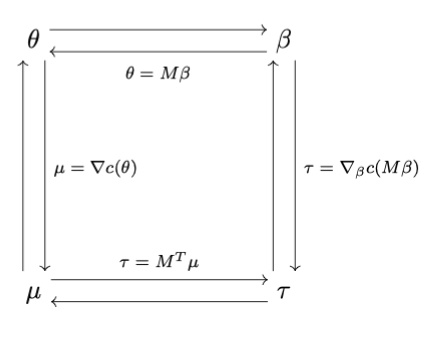
\includegraphics{transformations.png}
\end{frame}

\begin{frame}[fragile]{}
\protect\hypertarget{section-14}{}
We start with \[
  \langle M'y, \beta \rangle - c_\beta(\beta),
\] and then obtain \(\hat{\beta}\) by maximizing the above. From here:

\begin{itemize}
\tightlist
\item
  \(\hat{\theta} = M\hat{\beta}\)
\item
  \(\hat\mu = \nabla_\theta c(\theta^*)|_{\theta* = \hat{\theta}}\)
\item
  \(\hat\tau = M'\hat{u}\)
\end{itemize}

\vspace{12pt}

For example we can compute \(\hat\theta\) using the predict function or
by hand. \tiny

\begin{Shaded}
\begin{Highlighting}[]
\NormalTok{theta }\OtherTok{\textless{}{-}}\NormalTok{ m1}\SpecialCharTok{$}\NormalTok{x }\SpecialCharTok{\%*\%} \FunctionTok{coef}\NormalTok{(m1)}
\FunctionTok{head}\NormalTok{(}\FunctionTok{cbind}\NormalTok{(}\FunctionTok{predict}\NormalTok{(m1, }\AttributeTok{type =} \StringTok{"link"}\NormalTok{), theta), }\DecValTok{3}\NormalTok{)}
\end{Highlighting}
\end{Shaded}

\begin{verbatim}
##        [,1]      [,2]
## 1 -2.133881 -2.133881
## 2 -2.103061 -2.103061
## 3 -2.796665 -2.796665
\end{verbatim}
\end{frame}

\begin{frame}[fragile]{}
\protect\hypertarget{section-15}{}
The submodel canonical parameterization scale is bit awkward for
interpretation, although summary tables provide some insight to which
components of the submodel canonical parameter vector may be driving the
data generating process (under the assumed model).

\vspace{12pt}

R software provides functionality for estimating the mean value
parameters \[
  \text{E}(Y|X = x) = \mathbb{P}(Y = 1| X = x),
\]\\
associated with every individual in the study.

\vspace{12pt}
\tiny

\begin{Shaded}
\begin{Highlighting}[]
\NormalTok{p1 }\OtherTok{\textless{}{-}} \FunctionTok{predict}\NormalTok{(m1, }\AttributeTok{type =} \StringTok{"response"}\NormalTok{, }\AttributeTok{se.fit =} \ConstantTok{TRUE}\NormalTok{)}

\DocumentationTok{\#\# compute by hand}
\NormalTok{mu }\OtherTok{\textless{}{-}} \DecValTok{1}\SpecialCharTok{/}\NormalTok{(}\DecValTok{1} \SpecialCharTok{+} \FunctionTok{exp}\NormalTok{(}\SpecialCharTok{{-}}\NormalTok{theta))}
\FunctionTok{head}\NormalTok{(}\FunctionTok{cbind}\NormalTok{(p1}\SpecialCharTok{$}\NormalTok{fit, mu), }\DecValTok{3}\NormalTok{)}
\end{Highlighting}
\end{Shaded}

\begin{verbatim}
##         [,1]       [,2]
## 1 0.10584708 0.10584708
## 2 0.10879965 0.10879965
## 3 0.05750466 0.05750466
\end{verbatim}
\end{frame}

\begin{frame}[fragile]{Another point about model matrices}
\protect\hypertarget{another-point-about-model-matrices}{}
Recall that model \texttt{m1\_2} did not suppress the intercept.

\vspace{12pt}

This model's model matrix has the same span as the model that we have
been working with. Mean-value parameters are the same for both models.

\vspace{12pt}
\small

\begin{Shaded}
\begin{Highlighting}[]
\NormalTok{p1\_2 }\OtherTok{\textless{}{-}} \FunctionTok{predict}\NormalTok{(m1\_2, }\AttributeTok{type =} \StringTok{"response"}\NormalTok{, }\AttributeTok{se.fit =} \ConstantTok{FALSE}\NormalTok{)}
\FunctionTok{head}\NormalTok{(}\FunctionTok{cbind}\NormalTok{(p1}\SpecialCharTok{$}\NormalTok{fit, p1\_2), }\DecValTok{6}\NormalTok{)}
\end{Highlighting}
\end{Shaded}

\begin{verbatim}
##                    p1_2
## 1 0.10584708 0.10584708
## 2 0.10879965 0.10879965
## 3 0.05750466 0.05750466
## 4 0.10584708 0.10584708
## 5 0.14245614 0.14245614
## 6 0.14245614 0.14245614
\end{verbatim}
\end{frame}

\end{document}
